\section{Taxonomy of Semantic Search Approaches}
In this section, we identify the main dimensions in which existing solutions vary and then, provide a taxonomy of semantic search approaches.  

Search is about retrieving information that are relevant with respect to a given information need. Generally speaking, approaches that fall under the category of \emph{semantic search} use semantic data for representing information and (or) semantic models for interpreting the data and information needs. Generally, they can be defined in terms of the following main dimensions, i.e. 

\begin{itemize}
\item the \emph{type of information needs} targeted by the system,  
\item the representation of the information need called the \textit{query}, 
\item the representation of the underlying \textit{information} called \emph{data}, 
\item the \emph{semantic models} used to interpret query and data and 
\item the techniques for \emph{matching} the query against the data and for \emph{ranking} the results.  
\end{itemize}
	
A general overview of the types of information needs, queries, data, semantic models and matching and ranking techniques supported by existing semantic search approaches is illustrated in Fig.~\ref{}. We will now discuss these approaches along these different dimensions. 

\subsection{Information Needs}
Document search, entity search, factual search, relational search
 
\subsection{Queries}
Search is about end-user oriented interfaces: NL, keywords, facets

\subsection{Data}
Objects (documents, media and multimedia objects) with embedded semantic data, semantic datasets

\subsection{Semantic Models}
Linguistic models, conceptual models

\subsection{Matching \& Ranking Techniques}
Term-based, structure-based, semantic-based




%Generally, queries might be simple keywords, natural language or structured. Various kind of formal query languages have been proposed to formulate highly expressive (both in terms of structure and semantics) queries. Resources returned to the users range from text, audio and video up to multimedia documents. These documents embody different types of data, i.e. unstructured, semi-structured (in the form of RDF) that is not associated with a schema and fully structured data with a schema. Often, structured data available in Semantic Web languages such as RDF and OWL is also referred to as ``semantic data''.  Different matching framework are employed by these systems. IR systems primarily rely on features at the level of terms (language, words) whereas DB and KB systems exploit also the structure as well as the semantics for matching. On the other hand, while these DB and KB systems are concerned with producing precise matches (binary matching), IR systems rely on statistical methods that are inherently imprecise such that results are also associated with the degree of matching, i.e. IR systems perform imprecise matching and ranking. 
%
%Apart from these main aspects, semantic search systems can also be distinguished in terms of the notion of semantics that is employed for search.  
%
%\subsection{Semantic Models}
%Generally, semantics is concerned with the meaning of things. Meaning is established through a semantic model, which commonly captures interrelationships between elements and their interpretations. Various semantic models have been proposed and
%used in different research communities. The IR community typically relies on \textit{linguistic
%models} such as taxonomies and thesauri that capture relations between syntactical elements, i.e. words. In
%the database community, \textit{conceptual models} such as Entity Relationship (ER)
%diagrams are used to capture relations between entities
%\cite{DBLP:journals/tods/Chen76}. Thus, while linguistic models are concerned with meanings at the level of words, conceptual models more specifically deal with meanings at the level of real-world entities denoted by words. That is, conceptual models deal with interpretation of words in terms of real world entities the words refer to. Besides ER diagrams, conceptual models include less formal models such as semantic networks [cite] and very formal models such as logic-based theories, where interpretations are precise and computable \cite{DBLP:books/sp/StaabS04}.
% 
%In the Semantic Web community, \textit{ontologies} have received widespread acceptance. The notion of
%ontologies employed by this community is very general. Ontologies
%constitute rather a family of models, which might differ in the
%degree of expressiveness and formality, ranging from simple
%taxonomies and shallow conceptual model represented in RDF(S)
%to expressive formal models represented in Description Logics \cite{DBLP:books/sp/StaabS04}. Thus, ontologies include both linguistic and conceptual models. In practice, ontologies do not come only with the conceptual part but might also contain instances. In this sense, they are similar to databases (and knowledge bases) where the conceptual part corresponds to what is refer to as the schema (terminological knowledge) and instances correspond to the actual data of the database (assertional knowledge of the knowledge base).  
%
%\subsection{Semantic Search}
%As a general notion, a system essentially performs semantic search when a semantic model is employed. As illustrated in Fig. \ref{fig:semsearch}, a semantic model might be used to make sense of the data, to interpret the query and ultimately, to support matching that goes beyond the traditional term-based matching.  
%
%\begin{figure}
%	\centering
%		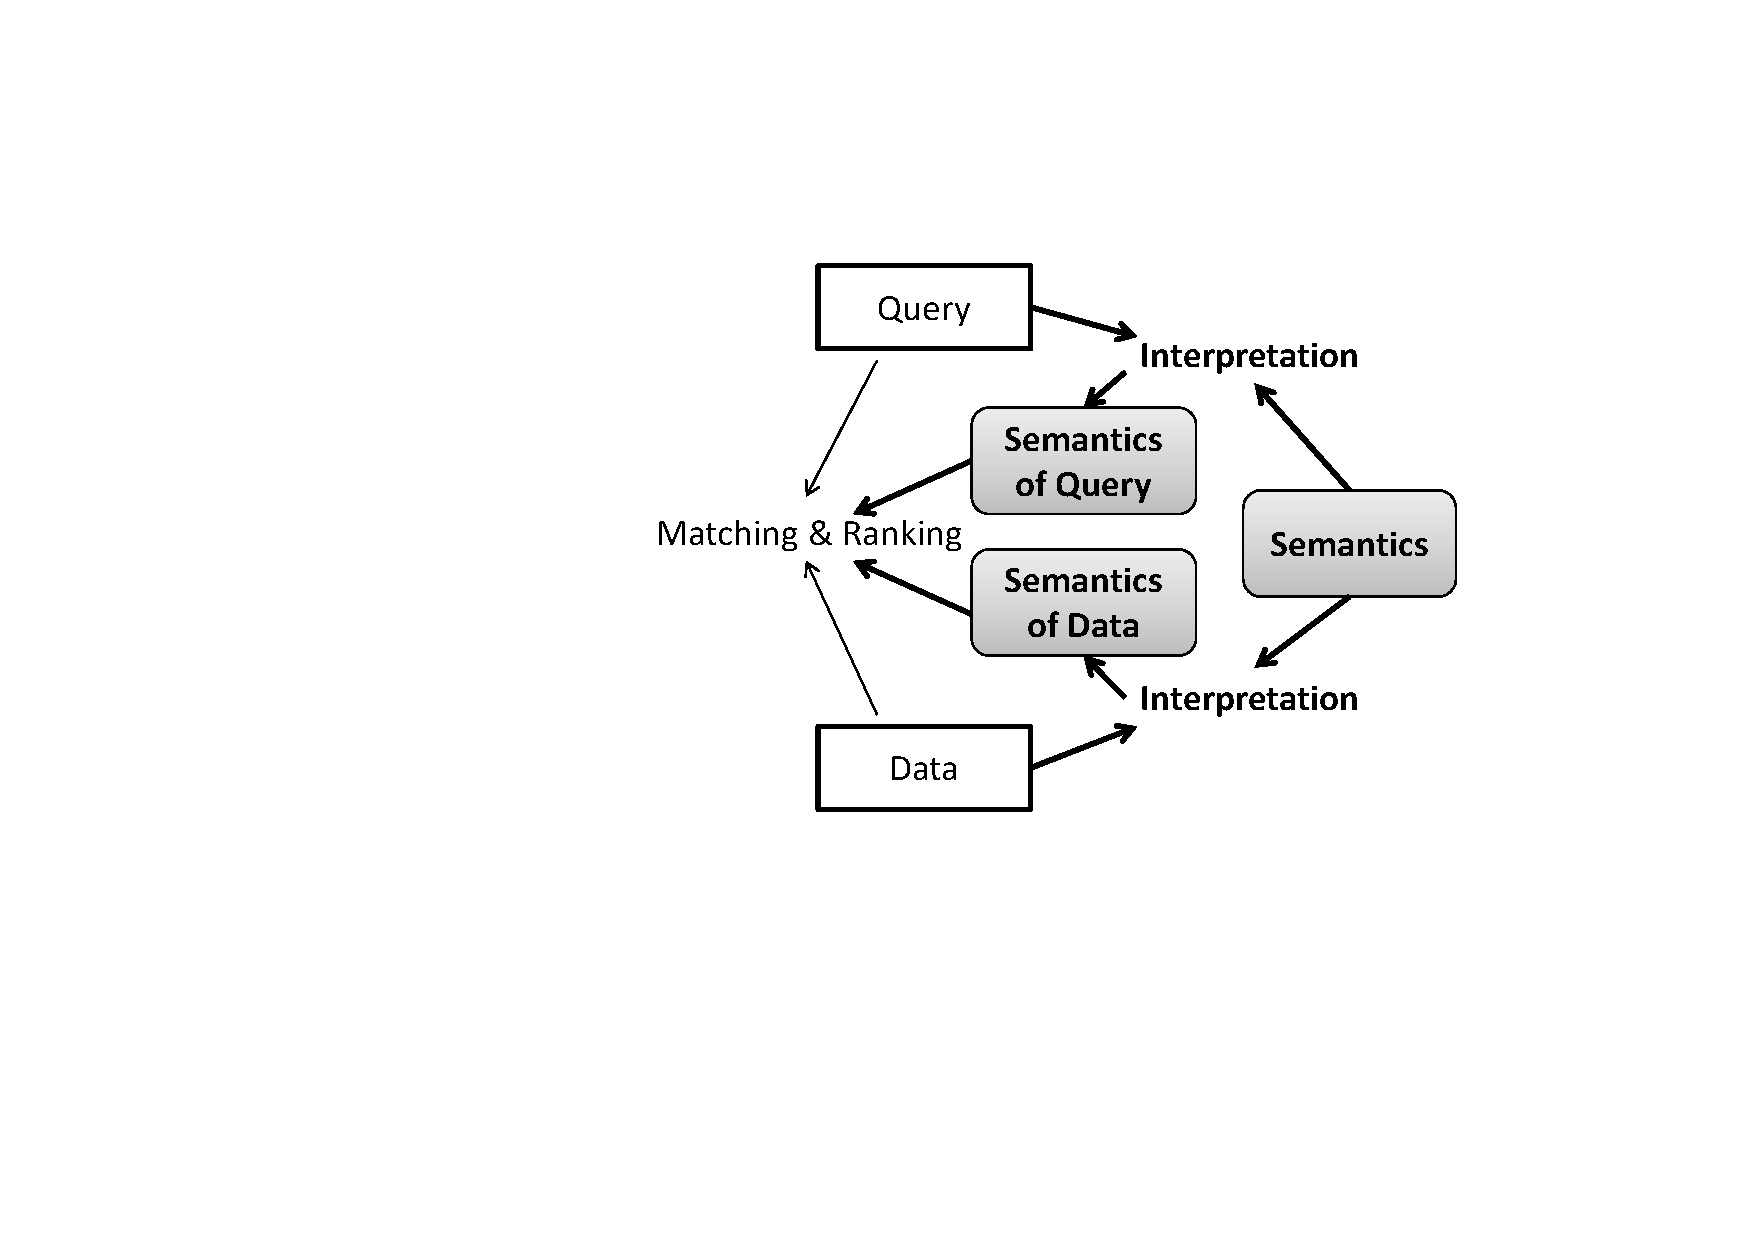
\includegraphics[width=0.5\textwidth]{figs/semsearch.pdf}
%	\label{fig:semsearch}
%	\caption{Semantic Search}
%\end{figure}
%
%\subsubsection{The DB\&KB Perspective}
%In retrieving data, semantics has always play an essential role in database systems. The foundation of database technologies manifested in theoretical models such as the relational model that provides formal semantics to both resources and queries, i.e. the model behind relational data and relational query (an important part of SQL) is in fact a fragment of first-order logic [cite]. This semantics is taken into account by database query engines to compute answers that precisely match the semantics of queries. More precisely, these engines perform binary matching that incorporates not only terms (i.e. constants) but also structure and semantics into account. Using this mechanism, information needs of different complexity have been served. In different commercial systems, we find the application of DB technologies in the form of simple product search (e.g. in commercial shopping sites like Ebay and Amazon) up to complex relational queries that are used to populate complex dynamic Web pages. 
%
%While the relational model is the one most widely used in practice, there exists also domain specific solutions that are built upon more expressive models. In the realm of deductive databases for instance, semantics represented in languages such Datalog or F-Logic is used to perform reasoning, with the goal of understanding and delivering not only explicitly asserted information, but also inferred one. Further down this steam, semantic models that are even more expressive are used by knowledge-based expert systems for answering complex questions. [TODO: applications of expert systems]
%
%
%\subsubsection{The IR Perspective}
%In the IR community, the representation of the information needs as well as resources is achieved primarily using lightweight models that operates at the level of words. In particular, the predominant paradigm is based on keyword queries and bag-of-words representation of resources. This works and most importantly, scales well for topical search, i.e. to retrieve documents based on topics expressed in terms of keywords, but is not sufficient to address the kind of complex information needs that can be served by DB and KB systems. 
%
%The need for going beyond the matching purely based on words and statistical dependencies that exist between them has been clearly expressed by leading researchers in the field. In the early years of IR research, Riksbergen clearly argue for the use of semantics. In order to return precise results to the user, it is essential to compute whether the resources semantically entail what the user ask for [cite]. Quoting a paper from W.B. Croft et al. published more than twenty years ago [cite]: ``The statistical approach has many advantages and can achieve a reasonable level of effectiveness with techniques that are very efficient. However, it appears that to achieve significant improvements in retrieval effectiveness compared to current techniques, systems must be designed to acquire and use explicit domain knowledge''. This explicit domain knowledge are captured using semantic models of varying degrees. Semantic networks have been used augment the models based on terms. This provide a richer representation which is exploited for assisted query formulation, query expansion, as well as for relevance propagation in ranking [cite].  Also, linguistic models particularly Wordnet and the Roget�s thesaurus have been widely used. 
%
%Recently, the IR community continues to embrace the vast body of explicit knowledge that increasingly, is made publicly available. There are approaches which not only use semantic models to enrich terms, but in fact, employ both the conceptual and the data part. In particular, there are systems that use ontologies including the semantic data contained in them [cite].   TODO: Applications: enterprise solutions such as IBM Avatar, Medline, Web solutions such as Hakia, Powerset. 
%
%
%\subsubsection{The SW Perspective}
%Semantic search from the this point of view is more similar to the DB and KB perspective in the sense that the main goal is to obtain precise answers for complex questions. However, while DB and KB systems are adopted to solve specific problems of a particular domain, semantics is taken by this community to the wider context of the Web. Semantic models used here are ontologies available in the W3C languages for resource description, namely RDF and OWL. 
%, while SPARQL is the primary mean to express information needs.
%On the Semantic Web, there is more data that is more hetetorogenous, i.e. data coming from different sources that differs in syntax, formats and quality. Thus, unlike traditional DB and KB systems, SW search engine are built with particular emphasis on the ability to scale in terms of both volume and the number of sources, to be domain independent and to perform ranking. 
%
%To achieve this, they are built upon concepts and technologies from database and expert systems. General concepts for data management (e.g. indexing and data partitioning []) as well as specific concepts for managing graph structured data and graph databases (e.g. structure indexes from XML databases []) have been adopted to deal with ontologies and semantic data available in RDF and OWL. For dealing with more expressive semantic models, techniques commonly applied in deductive databases (e.g. magic set optimizations [cite]) have been adopted to improve the efficiency and scalability of reasoning. However, to deal with scale and to perform ranking, techniques that are more commonly used by the IR technology has also been adopted. For instance, the inverted index has been used to scale to a large amount of data and to support term-based matching. Statistical dependencies of words such TF-IDF as well as authority-based metrics such as PageRank that is popular in IR web search engines, have been used for ranking. 
%
%TODO: Applications
%
%
%
%To summarize, semantics has proven to be useful for search in many aspects. There are commercial exploitations, which used semantics in different ways. Thus, the notion of semantic search is thus very broad. Semantic search covers the wide range of systems employing and exploiting semantic models of varying expressiveness. In the following sections, we will focus on semantic search systems driven by the IR and the SW communities which recently, have attracted much research and commercial interests. 

